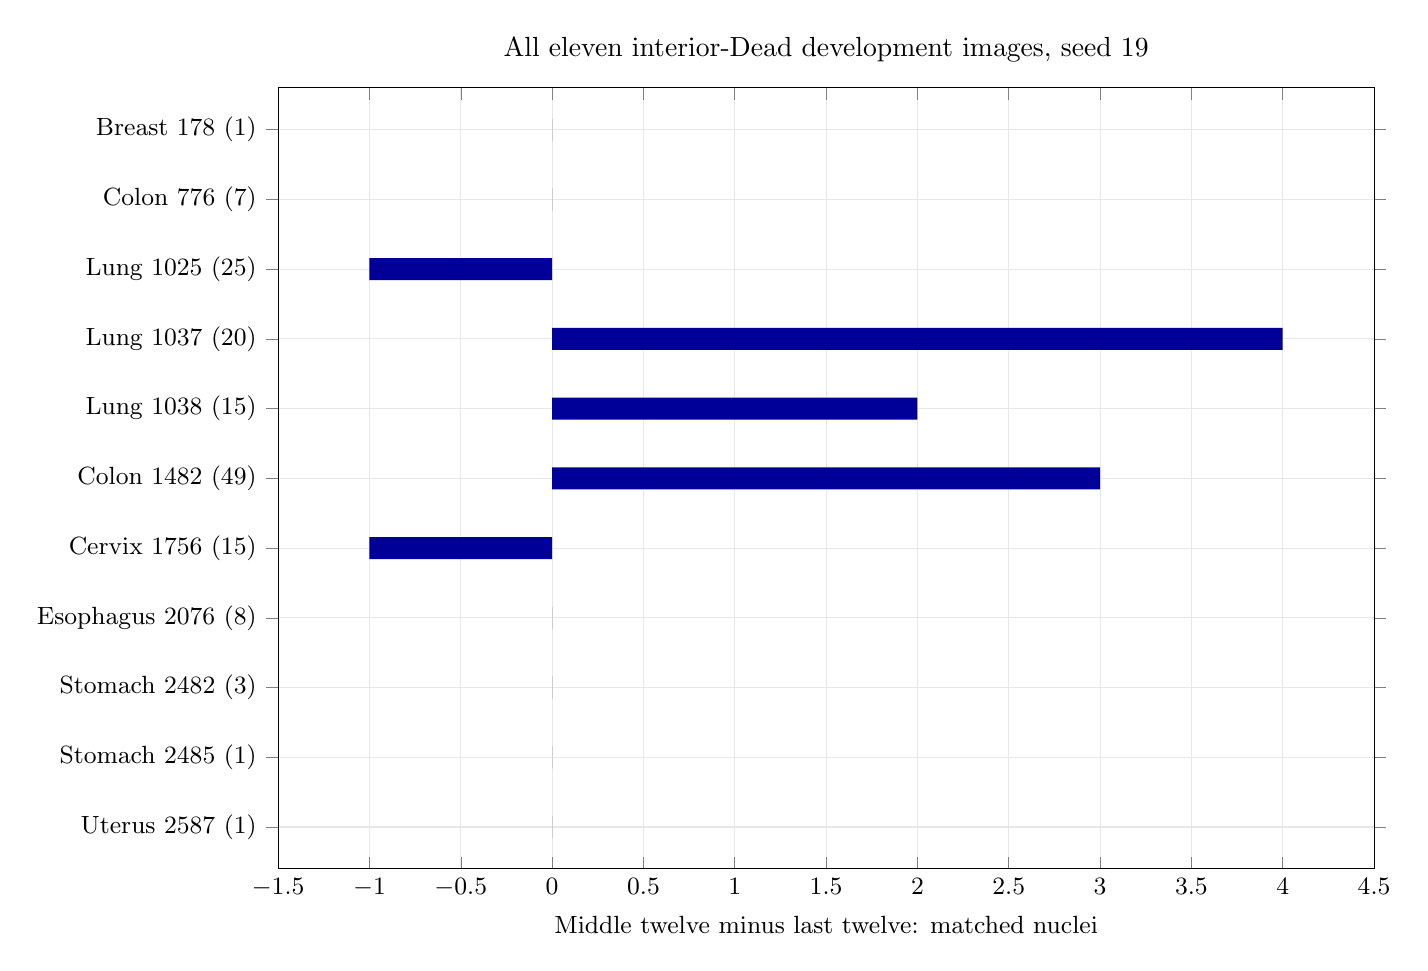
\begin{tikzpicture}
\begin{axis}[xbar,width=15.5cm,height=11.5cm,xlabel={Middle twelve minus last twelve: matched nuclei},title={All eleven interior-Dead development images, seed 19},ytick={0,1,2,3,4,5,6,7,8,9,10},yticklabels={{Breast 178 (1)},{Colon 776 (7)},{Lung 1025 (25)},{Lung 1037 (20)},{Lung 1038 (15)},{Colon 1482 (49)},{Cervix 1756 (15)},{Esophagus 2076 (8)},{Stomach 2482 (3)},{Stomach 2485 (1)},{Uterus 2587 (1)}},ymin=-.6,ymax=10.6,y dir=reverse,bar width=8pt,grid=major,grid style={gray!18},tick label style={font=\small},label style={font=\small},title style={font=\normalsize}]
\addplot[fill=blue!60!black,draw=none] coordinates {(0,0) (0,1) (-1,2) (4,3) (2,4) (3,5) (-1,6) (0,7) (0,8) (0,9) (0,10)};
\end{axis}
\end{tikzpicture}
